\documentclass[tikz]{standalone}
\begin{document}
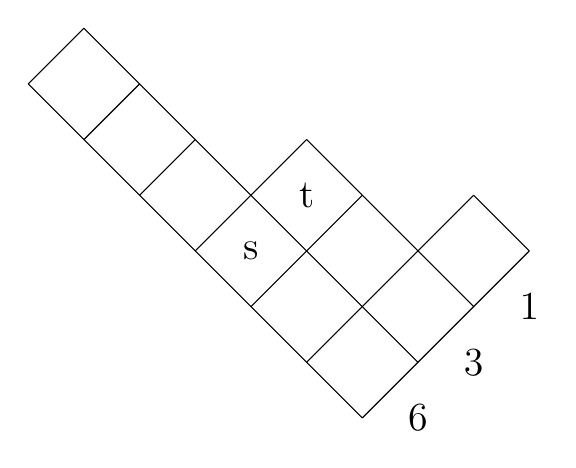
\begin{tikzpicture}
\begin{scope}[scale=0.7071, font=\Large]
\draw (0,0) -- (-6,6);\draw (1,1) -- (-5,7);\draw (1, 0) node{6};\draw (2,2) -- (-1,5);\draw (2, 1) node{3};\draw (3,3) -- (2,4);\draw (3, 2) node{1};\draw (0,0) -- (3,3);\draw (-1,1) -- (2,4);\draw (-2,2) -- (0,4);\draw (-3,3) -- (-1,5);\draw (-4,4) -- (-3,5);\draw (-5,5) -- (-4,6);\draw (-6,6) -- (-5,7);
\draw (-2, 3) node{s};\draw (-1, 4) node{t};
\end{scope}
\end{tikzpicture}
\end{document}
